\section{Developer Documentation}
\label{sec:devdocs} 

\subsection{Prerequisites}

In order to do development work on \emph{Colonizers}, the following software
is required:
\begin{itemize}
    \item .NET Core 3.1 SDK
    \item Python 3.7
    \item Node.js 10 and NPM 6.4.1
\end{itemize}
The game's UI is designed for a minimum screen resolution of 1920x1080 at
100\% zoom level. It is not recommended to play the game on lower resolution
screens, since graphical errors may occur.

In order to build and run \emph{Colonizers} in Electron, the Electron.NET CLI
package is required. You may install this package as a .NET Core tool by running
the \texttt{dotnet tool install ElectronNET.CLI -g} command. This gives you
access to the \texttt{electronize} command.

It is also highly recommended to use Visual Studio 2019 for development work
on the game engine or the UI. Visual Studio 2019 provides support for debugging
both the UI and the game engine in the same window, which makes for a~seamless
development experience. Visual Studio 2019 is also capable of attaching
to an external process for debugging, which turns out to be
extremely useful with Electron.NET.

For developing and debugging Python AI scripts, the author used Visual Studio Code,
but other software capable of debugging Python scripts is viable as well.

\subsection{Project Structure}

The entire game is contained in a .sln (solution) file, which is a file type used
to organize projects in Visual Studio. This solution contains four projects:
\begin{itemize}
    \item \texttt{AICore} --- project with the API for AI scripts and the AICore
        scripts themselves.
    \item \texttt{Desktop} --- project with the UI, consisting of an~Angular
        web application and an ASP.NET Core Web API. The Web API is the
        \emph{ClientApp} subfolder of this project's folder.
    \item \texttt{Game} --- C\# library project containing the game logic
        and code responsible for communicating with Python AIs.
    \item \texttt{Experiments} --- console application project containing
        the experiment scenarios explored in this thesis.
\end{itemize}

The flow of data in the application starts with the UI, since all initiative starts
with the user. The UI then uses the ASP.NET Core Web API to execute game logic.
If required, game logic then talks to processes executing Python AI sripts.
This flow can be seen in \Cref{dd:sequence}.

\begin{figure}[ht]
\centerline{\mbox{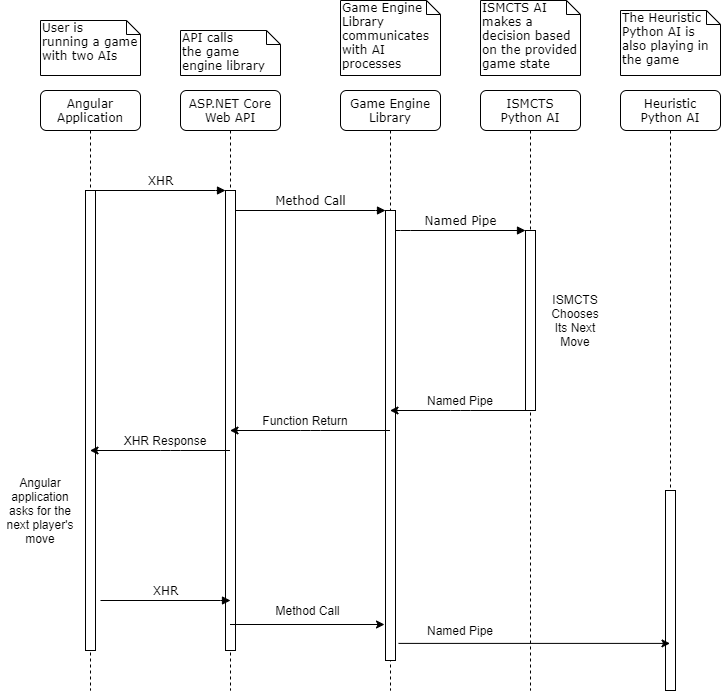
\includegraphics[width=130mm]{colonizers-sequence}}}
\caption{\emph{Colonizers} sequence diagram.}\label{dd:sequence}
\end{figure}

The aforementioned components will be discussed in more detail in the following subsections.

\subsection{Game Engine}

WORK IN PROGRESS

\subsection{Artificial Intelligence}
\label{chap:aidev}

WORK IN PROGRESS

\subsection{User Interface}

\emph{Colonizers} uses Electron as a means to run the game as a desktop application,
since the game is developed using web technologies. Specifically, it uses the
Electron.NET library, which provides an access to the Electron APIs to C\# applications,
and it also facilitates usage of Electron's build tools to package C\# applications.
C\# and the whole .NET platform in general still do not have a widely-used cross-platform
UI framework, therefore Electron was a good fit for this project.

The UI for \emph{Colonizers} is an Angular application, which is then served inside
Electron. Electron then uses the Chromium rendering engine and Node.js in the background.
The Angular application allows configuration of the game, it handles presentation
of game state to the user, and it is responsible for communicating with the
ASP.NET Core Web API.

\subsection{Experiments}
\label{chap:experimentdocs}

The experiments performed in this thesis are implemented in the \texttt{Experiments}
project of the \texttt{Colonizers} solution. It is a C\# console application project.
It is invoked via the command line with two arguments --- the first is a~number
between 1 and 5, corresponding to the experiment number, and the second
is the path to the Python executable to use when executing AI scripts.

% TODO: verify where the JSON file is generated
After the experiment is run, it will produce a JSON file containing the results
of the experiment. This file is generated in the directory where the experiments
are running.
\Cref{dd:experimentjson} shows the structure of these JSON files, with less
important fields omitted for brevity. The JSON files associated with the five
experiments are also located in the \texttt{Experiments} projects, namely in
the \texttt{Results} folder. They were added there for reference, since
some experiments may take tens of hours to run even on reasonably fast
machines. Be aware that a simple diff of the JSON result files
is not sufficient for determining whether or not a given experiment was successfully
replicated. This is because the files contain running times of the games as well.

\begin{figure}[ht]
\begin{code}[commandchars=\\\{\},codes={\catcode`\$=3\catcode`\^=7\catcode`\_=8}]
$\{$
    "Players": [
        "Name": "ISMCTS",
        "PlayerEndInfo": $\{$
            "Ranking": 3,
            "VictoryPoints": 24,
            "Player": $\{$
                "ID": 1,
                ...
            $\}$
        $\}$
    ],
    "Duration": "00:12:28.1879334"
$\}$
\end{code}
\caption{Experiment result JSON file structure (simplified).}\label{dd:experimentjson}
\end{figure}

The class \texttt{Scenarios} contains the setup for the experiments,
and each scenario then calls \texttt{ExperimentRunner} to performed
the experiment itself.

A noteworthy point is the implementation of the shuffling of players between games.
Since the game engine already possessed an implementation of the Fisher-Yates Shuffle
\cite{Knuth98} for shuffling lists, this implementation was reused for shuffling the
players themselves. This means that if we were to run the experiments
without shuffling, and instead assigning the players the same positions they would
have been assigned by the shuffle, the results of this experiment would be different.
This is because running the shuffle manipulates the game engine's random number generator.
